\section{Experiments}
\label{sec:exp}

\begin{table*}[t]
\caption{\textbf{Results (\%) on ImageNet-R}. Results are included for 5 tasks (40 classes per task), 10 tasks (20 classes per task), and 20 tasks (10 classes per task). $A_N$ gives the accuracy averaged over tasks and $F_N$ gives the average forgetting. We report results over 5 trials. %
}
\label{tab:imnet-r_main}
\centering

\begin{tabular}{c||c c||c c||c c} 
\hline 
Tasks & \multicolumn{2}{c||}{5} & \multicolumn{2}{c||}{10} & \multicolumn{2}{c}{20} \\
\hline
\rule{0pt}{10pt} Method & $A_N$ ($\uparrow$) & $F_N$ ($\downarrow$) & $A_N$ ($\uparrow$) & $F_N$ ($\downarrow$) & $A_N$ ($\uparrow$) & $F_N$ ($\downarrow$) \\
\hline
UB  
& $77.13$ & - 
& $77.13$ & - 
& $77.13$ & -   \\ 
\hline
ER (5000)        
& $71.72 \pm 0.71$ & $13.70 \pm 0.26$ 
& $64.43 \pm 1.16$ & $10.30 \pm 0.05$
& $52.43 \pm 0.87$ & $7.70 \pm 0.13$  \\  
FT          
& $18.74 \pm 0.44$ & $41.49 \pm 0.52$
& $10.12 \pm 0.51$ & $25.69 \pm 0.23$
& $4.75 \pm 0.40$ & $16.34 \pm 0.19$  \\
FT++          
& $60.42 \pm 0.87$ & $14.66 \pm 0.24$
& $48.93 \pm 1.15$ & $9.81 \pm 0.31$
& $35.98 \pm 1.38$ & $6.63 \pm 0.11$  \\
LwF.MC       
& $74.56 \pm 0.59$ & $4.98 \pm 0.37$ 
& $66.73 \pm 1.25$ & $3.52 \pm 0.39$
& $54.05 \pm 2.66$ & $2.86 \pm 0.26$  \\
L2P++        
& $70.83 \pm 0.58$ & $3.36 \pm 0.18$
& $69.29 \pm 0.73$ & $2.03 \pm 0.19$ 
& $65.89 \pm 1.30$ & $1.24 \pm 0.14$   \\
Deep L2P++  
& $73.93 \pm 0.37$ & $2.69 \pm 0.10$
& $71.66 \pm 0.64$ & $1.78 \pm 0.16$ 
& $68.42 \pm 1.20$ & $1.12 \pm 0.13$  \\
DualPrompt 
& $73.05 \pm 0.50$ & $\bm{2.64 \pm 0.17}$
& $71.32 \pm 0.62$ & $1.71 \pm 0.24$ 
& $67.87 \pm 1.39$ & $1.07 \pm 0.14$   \\
\hdashline
\textbf{CODA-P-S} 
& $75.19 \pm 0.47$ & $2.65 \pm 0.15$
& $73.93 \pm 0.49$ & $1.60 \pm 0.20$
& $70.53 \pm 1.24$ & $1.00 \pm 0.15$  \\
\textbf{CODA-P}   
& $\bm{76.51 \pm 0.38}$ & $2.99 \pm 0.19$
& $\bm{75.45 \pm 0.56}$ & $\bm{1.64 \pm 0.10}$
& $\bm{72.37 \pm 1.19}$ & $\bm{0.96 \pm 0.15}$  \\ 

\hline
\end{tabular}
\end{table*}








We benchmark our approach with several image datasets in the class-incremental continual learning setting. We implemented baselines which do not store training data for rehearsal: Learning without Forgetting (LwF)~\cite{li2016learning}, Learning to Prompt (L2P)~\cite{wang2022learning}, and DualPrompt~\cite{wang2022dualprompt}. Additionally, we report the upper bound performance (i.e., trained offline) and performance for a neural network trained only on classification loss using the new task training data (we refer to this as FT), and include an improved version of FT which uses the same classifier implementation\footnote{See \SMa{} for additional details} as L2P/DualPrompt (referred to as FT++). We also compare to Experience Replay~\cite{chaudhry2019tiny} to provide additional context to our results. We implement our method and all baselines in PyTorch\cite{paszke2019pytorch} using the ViT-B/16 backbone~\cite{dosovitskiy2020image} pre-trained on ImageNet-1K~\cite{russakovsky2015imagenet}. Our contribution includes faithful PyTorch implementations of the popular prompting baselines L2P and DualPrompt, which were released in JAX\cite{wang2022dualprompt,wang2022learning}. Our implementations of the competing methods actually achieve slight boosts in the performance of DualPrompt in most benchmarks, as well as significant performance boosts in L2P due to the improved prompting type\footnote{As discussed in Section~\ref{sec:prelim_b}, we use pre-fix tuning over prompt-tuning for all implementations as is shown to work best for continual learning~\cite{wang2022dualprompt}.} (which we refer to as L2P++). 


DualPrompt uses length 5 prompts in layers 1-2 (referred to as \emph{general} prompts) and length 20 prompts in layers 3-5 (referred to as \emph{task-expert}) prompts.  We insert prompts into the same layers as DualPrompt (layers 1-5) for CODA-P 
and use a prompt length of 8 and 100 prompt components, which were chosen with a hyperparameter sweep on validation data to have the best trade-off between performance and parameter efficiency. Because our approach introduces more learnable parameters compared to DualPrompt, we include a variant of out method \textbf{CODA-P-S} which uses a smaller number of parameters equal to DualPrompt for additional comparison. We show that our method outperforms other methods even under this condition, while still retaining the capability to scale if desired.

We report results on the test dataset, but emphasize that all hyperparameters and design decisions (including for the baselines) were made using validation data (20\% of the training data). Unlike DualPrompt, we run our benchmarks for several different shuffles of the task class order and report the mean and standard deviation of these runs. We do this with a consistent seed (different for each trial) so that results can be directly compared. This is crucial because the results with different shuffling order can be different due to differences in task difficulty and their appearance order. \emph{We include additional implementation details and results in \SMb{}}.


\noindent
\textbf{Evaluation Metrics:} We evaluate methods using (1)
average final accuracy $A_{N}$, or the final accuracy with respect to all past classes averaged over $N$ tasks, and (2) average forgetting~\cite{chaudhry2018efficient,Lopez-Paz:2017,mai2022online} $F_{N}$, or the drop in task performance averaged over $N$ tasks. The reader is referred to \SMc{} for additional details about these metrics. We emphasize that $A_{N}$ is the more important metric and encompasses both method plasticity \emph{and} forgetting, whereas $F_{N}$ simply provides additional context.


\begin{table*}[t]
\caption{\textbf{Results (\%) on CIFAR-100 and DomainNet}. $A_N$ gives the accuracy averaged over tasks and $F_N$ gives the average forgetting. We report results over 5 trials for CIFAR-100 and 3 trials for DomainNet (due to dataset size).}
\begin{subtable}[h]{0.49\textwidth}
\centering
\caption{10-task CIFAR-100 (10 classes per task)}
\label{tab:cifar}
\begin{tabular}{c||c c} 
\hline
\rule{0pt}{10pt} Method  & $A_N$ ($\uparrow$) & $F_N$ ($\downarrow$)  \\
\hline
Upper-Bound & $89.30$ & -  \\  
\hline
ER (5000) & $76.20 \pm 1.04$ & $8.50 \pm 0.37$ \\ 
FT        & $9.92 \pm 0.27$ & $29.21 \pm 0.18$   \\  
FT++      & $49.91 \pm 0.42$ & $12.30 \pm 0.23$   \\ 
LwF.MC    & $64.83 \pm 1.03$ & $5.27 \pm 0.39$   \\ 
L2P++     & $82.50 \pm 1.10$ & $1.75 \pm 0.42$   \\
Deep L2P++ & $84.30 \pm 1.03$ & $\bm{1.53 \pm 0.40}$ \\  
DualPrompt & $83.05 \pm 1.16$ & $1.72 \pm 0.40$  \\
\hdashline
\textbf{CODA-P-S}& $84.59 \pm 0.87$ & $1.76 \pm 0.28$  \\
\textbf{CODA-P}   & $\bm{86.25 \pm 0.74}$ & $1.67 \pm 0.26$   \\

\hline
\end{tabular}

\end{subtable}
\hfill
\begin{subtable}[h]{0.49\textwidth}
\centering
\caption{5-task DomainNet (69 classes per task)}
\label{tab:domainnet}
\begin{tabular}{c||c c} 
\hline
\rule{0pt}{10pt} Method  & $A_N$ ($\uparrow$) & $F_N$ ($\downarrow$) \\
\hline
Upper-Bound  & $79.65$ & -   \\  
\hline
ER (5000)   & $58.32 \pm 0.47$ & $26.25 \pm 0.24$  \\
FT          & $18.00 \pm 0.26$ & $43.55 \pm 0.27$    \\ 
FT++        & $39.28 \pm 0.21$ & $44.39 \pm 0.31$   \\ 
LwF.MC      & $\bm{74.78 \pm 0.43}$ & $5.01 \pm 0.14$ \\
L2P++       & $69.58 \pm 0.39$ & $2.25 \pm 0.08$  \\
Deep L2P++  & $70.54 \pm 0.51$ & $2.05 \pm 0.07$   \\ 
DualPrompt  & $70.73 \pm 0.49$ & $\bm{2.03 \pm 0.22}$  \\
\hdashline
\textbf{CODA-P-S}   & $71.80 \pm 0.57$ & $2.54 \pm 0.10$  \\
\textbf{CODA-P}     & $73.24 \pm 0.59$ & $3.46 \pm 0.09$  \\

\hline
\end{tabular}

\end{subtable}

\end{table*}













\subsection{CODA-P sets the SOTA on existing benchmarks}
We first evaluate our method and state of art on several well-established benchmarks. Table~\ref{tab:imnet-r_main} provides results for ImageNet-R~\cite{hendrycks2021many,wang2022dualprompt} which is composed of 200 object classes with a wide collection of image styles, including cartoon, graffiti, and hard examples from the original ImageNet dataset~\cite{russakovsky2015imagenet}. This benchmark is attractive because the distribution of training data has significant distance to the pre-training data (ImageNet), thus providing a fair and challenging problem setting. In addition to the original 10-task benchmark, we also provide results with a smaller number of large tasks (5-task) and a larger number of small tasks (20 task). We first notice that our reported performance for DualPrompt is a few percentage points higher compared to the original DualPrompt~\cite{wang2022dualprompt} paper. We re-implemented the method from scratch in a different framework (PyTorch~\cite{paszke2019pytorch}) and suspect the difference has to do with our averaging over different class-order shuffling. 
We note that our implementation of L2P (L2P++) performs significantly better than originally reported because we use the same form of prompting as DualPrompt (for fair comparison). Furthermore, our ``Deep L2P ++", which prompts at the same 5 layers as DualPrompt (rather than only at layer 1), actually performs similarly to DualPrompt.

\looseness=-1
Importantly, we see that our method has strong gains in average accuracy across all three task lengths, with as much as \textbf{4.5\% improvement in average accuracy over DualPrompt}. We remind the reader that CODA-P is our proposed method with tuned prompt length and component set size, whereas CODA-P-S is downsized (see \SMd{} for exact details) to exactly match the number of learnable parameters as DualPrompt. We notice that our method often has slightly higher average forgetting compared to DualPrompt. Given that average accuracy is the crucial metric that captures practical performance, we are not worried by the slight uptick in forgetting. In fact, we argue it is very reasonable and reflects the strength of our approach: our method has a larger capacity to learn new tasks, and thus we can sacrifice marginally higher forgetting. Crucially, we see that as the task sequence length grows, the forgetting metric of our method versus DualPrompt begin to converge to a similar value. 

We provide results for experience replay to provide additional context of our results. While the gap between rehearsal with a substantial coreset size (i.e., the buffer size of replay data) and our approach is small for the short task sequence, we see that our method strongly outperforms rehearsal in the longer task sequence.

\looseness=-1 Tables~\ref{tab:cifar}~and~\ref{tab:domainnet} provide results on additional\footnote{Note that the hyperparameters for both DualPrompt and CODA-P were tuned on ImageNet-R, which was intentionally done to evaluate robustness of all methods.} benchmarks ten-task CIFAR-100~\cite{krizhevsky2009learning} and five-task DomainNet~\cite{peng2019moment}. While neither dataset is as impactful as ImageNet-R in terms of challenge and distance from the pre-trained distribution, these tables provide additional context to our method's performance. 
These tables illustrate a similar story to the ImageNet-R benchmarks, with improvements of +3.2\% and +2.5\%, respectively. We do note that, surprisingly, LwF~\cite{li2016learning} slightly outperforms prompting on this benchmark.

\subsection{CODA-P sets the SOTA for a new dual-shift benchmark}

We also evaluate on a challenging \emph{dual-shift} benchmark using the ImageNet-R dataset. Our motivation is to show robustness to two different types of continual distribution shifts: semantic \emph{and} covariate. We accomplish this by randomly selecting image types from the ImageNet-R dataset to include in each task's training data (while keeping the evaluation data unmodified). The reader is refereed to \SMe{} for more details. Results for this benchmark are provided in Table~\ref{tab:imnet-r_domainshift}. Compared to 5-task ImageNet-R where our method improves SOTA by 4.5\% average accuracy, we see a 4.4\% improvement on this 5-task benchmark with similar forgetting margins. Our results indicate that CODA-P better generalizes to real-world type shifts.%



\subsection{Ablations and Additional Analysis}

\label{section:exp_ablations_analysis}

We take a closer look at our method with ablation studies and additional analysis. In Table~\ref{tab:ablations} we show the effect of removing a few key components of our method: attention keys, freezing of past task components, and our orthogonality regularization. We show that removing attention slightly reduces forgetting degrades performance on average accuracy (the more important metric). This makes sense because removing the attention keys makes our query processing more aligned with the L2P/DualPrompt methods which boast low forgetting but lack sufficient learning capacity. We see larger drops when removing freezing and orthogonality. This indicates that these aspects are crucial to our approach. Our intuition is is that, without these, our prompt formation is similar to a shallow MLP module which, unregularized, should suffer from high forgetting.
\begin{table}[t]
\caption{\textbf{Results (\%) on ImageNet-R \emph{with covariate domain shifts}}. Results are included for 5 tasks (40 classes per task). We simulate domain shifts by randomly removing 50\% of the dataset's domains (e.g., clipart, paintings, and cartoon) for the training data of each task (see SM for more details). $A_N$ gives the accuracy averaged over tasks and $F_N$ gives the average forgetting. We report results over 5 trials.}

\centering
\label{tab:imnet-r_domainshift}
\begin{tabular}{c||c c} 
\hline
\rule{0pt}{10pt} Method & $A_N$ ($\uparrow$) & $F_N$ ($\downarrow$) \\
\hline
Upper-Bound   & $77.13$ & $2.66$   \\ 
\hline
ER (5000)    & $67.39 \pm 0.37$ & $11.94 \pm 0.17$  \\
FT           & $17.93 \pm 0.27$ & $37.49 \pm 0.28$ \\
FT++         & $54.51 \pm 0.68$ & $14.41 \pm 0.33$ \\
LwF.MC       & $64.02 \pm 1.55$ & $7.05 \pm 0.27$  \\
L2P++        & $65.08 \pm 0.29$ & $2.79 \pm 0.32$  \\
Deep L2P++   & $65.74 \pm 0.12$ & $2.48 \pm 0.30$   \\ 
DualPrompt   & $66.98 \pm 0.08$ & $\bm{2.21 \pm 0.28}$   \\
\hdashline
\textbf{CODA-P-S}   & $69.73 \pm 0.18$ & $2.35 \pm 0.19$  \\
\textbf{CODA-P}     & $\bm{71.35 \pm 0.08}$ & $2.56 \pm 0.26$  \\

\hline
\end{tabular}
\end{table}





\begin{table}[t]
\caption{\textbf{Ablation Results (\%) on 10-task ImageNet-R}. $A_N$ gives the accuracy averaged over tasks and $F_N$ gives the average forgetting. We report results over 5 trials.}

\centering
\label{tab:ablations}

\begin{tabular}{c||c|c} 
\hline
\rule{0pt}{10pt} Method & $A_N$ ($\uparrow$) & $F_N$ ($\downarrow$) \\
\hline
CODA-P               & $75.45 \pm 0.56$ & $1.64 \pm 0.10$   \\ 
\hline
Ablate Attention     & $74.52 \pm 0.65$ & $1.67 \pm 0.13$   \\  
Ablate Freezing      & $74.60 \pm 0.64$ & $2.29 \pm 0.10$   \\ 
Ablate Orthogonality & $70.66 \pm 0.60$ & $1.74 \pm 0.25$   \\ 

\hline
\end{tabular}
\end{table}

\begin{figure}[t]
    \centering
    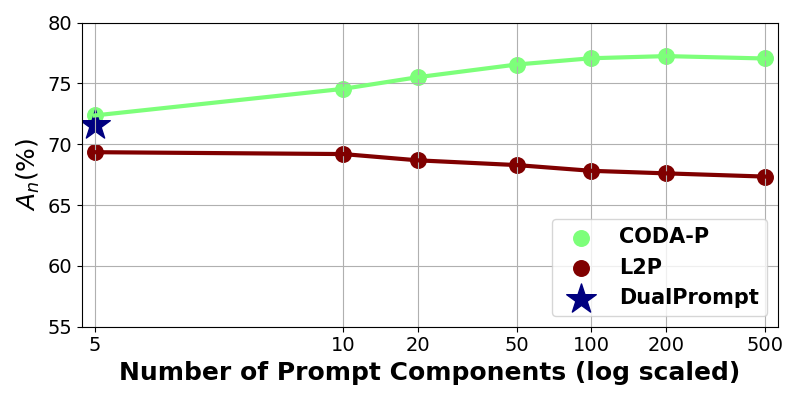
\includegraphics[width=0.4\textwidth]{figures/source/cvpr-pool-sweep.png}
    \caption{\textbf{Analysis of average accuracy $A_N$ vs prompt components (or pool size)} for CODA-P, L2P, and DualPrompt. The setting is 5 task ImageNet-R, and we report the mean over 3 trials.}
    \label{fig:capacity}
\end{figure}

\begin{figure}[t]
    \centering
    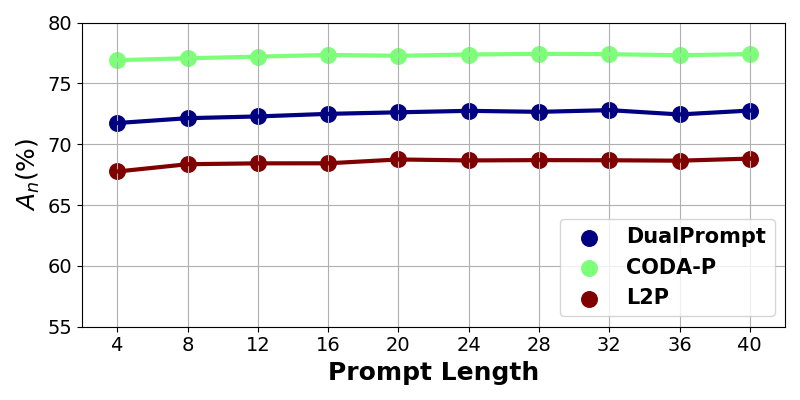
\includegraphics[width=0.4\textwidth]{figures/source/cvpr-len-sweep.png}
    \caption{\textbf{Analysis of average accuracy $A_N$ vs prompt length} for CODA-P, L2P, and DualPrompt. The setting is 5 task ImageNet-R, and we report the mean over 3 trials.}
    \label{fig:len}
\end{figure}


\looseness=-1
We also look at our ability to grow in model capacity along our newly introduced prompt component dimension using the 5-task ImageNet-R benchmark (with validation data). We show in Figure~\ref{fig:capacity} that, with a number of prompt components equal to the number of prompts learned in DualPrompt, we achieve higher performance. Importantly, when we increase the number of components, we are able to leverage the scaled parameters for significantly higher performance, finding that our method is closer to upper bound performance than it is to DualPrompt in average accuracy. Because the prompt pool in L2P can be increased to arbitrary size as well, we include results in this analysis as well. However, we show that the L2P method peaks with a pool size equal to twice the task sequence length, and then drops in performance. This reflects that our \emph{prompt components} benefit from scale, whereas the existing \emph{prompt pool} actually suffer. 

\looseness=-1
Finally, we show average accuracy versus prompt \emph{length} in Figure~\ref{fig:len} using the same setting as above. The purpose of this experiment is to emphasize that \emph{accuracy saturates with prompt length}, thus motivating the need to expand in our introduced \emph{component} dimension.
\emph{Additional analysis and hyperparameter sweeps is available in \SMf{}.}
